\documentclass{article}
\RequirePackage[T1]{fontenc}
\usepackage[screen]{tuepdfscreen}
\usepackage{graphicx, fleqn, tabularx, wrapfig}
\usepackage[ansinew]{inputenc}
\usepackage[spanish]{babel}

\hypersetup{
  pdfauthor={Antalcides Olivo},
  pdftitle={INDUCCI�N AL LABORATORIO },
  pdfsubject={pdfscreen},
  pdfkeywords={pdfscreen,hyperref,presentaties,presentations,slides,latex,miktex},
  pdfpagemode={FullScreen}
}

%%
%% Navigation buttons at the bottom
%%
\bottombuttons
%%
%% Page numbers at the bottom
%%
\pagenumbering
%%
%% Background image
%%
\overlay{tuebgkuk}

\title{\Huge F�sica Calor Ondas\\\Large Laboratorio}
\author{\Large Universidad Del Norte}
\date{\large 12 de agosto del 2003}

\begin{document}

\newenvironment{descrsf}[1]
  {\begin{list}{}{\renewcommand{\makelabel}[1]{\textsf{##1}\hfil}
                  \setlength{\itemsep}{0.5em}
                  \setlength{\parsep}{0pt}
                  \settowidth{\labelwidth}{\textsf{#1}}
                  \setlength{\labelsep}{10pt}
                  \setlength{\leftmargin}{\labelwidth}
                  \addtolength{\leftmargin}{\labelsep}
                 }
  }
  {\end{list}}

\renewcommand{\descriptionlabel}[1]%
   {\hspace{\labelsep}\textsf{#1}}

\begin{slide}
\maketitle
\end{slide}

\begin{slidetop}
\setlength{\parskip}{0.5cm}
\section{Introduction}
La idea de esta inducci�n es recordar como utilizar el software
Data Studio como herramienta para interpretar fen�menos f�sicos y
obtener resultados acorde con la teor�a dada en clase, adem�s
explicaremos como realizar ajuste de datos a curvas y realizar
c�lculos de error e interpretarlos


\begin{slidetop}
\section{Adobe Acrobat Shortcut Keys}

It is quite useful to know (some of) these shortcut keys in Adobe Acrobat Reader:

\begin{descrsf}{PAGE DOWN}
\item[PAGE UP] go back to the previous slide
\item[PAGE DOWN] advance to the next slide
\item[HOME] go to the first slide
\item[END] go to the last slide
\item[CTRL+L] toggle between Full Screen mode and normal viewing mode
\item[CTRL+N] prompts for a page number and opens that page
\item[CTRL+P] brings up the print dialog
\item[F8, F9] toggle visibility menu bar and tool bar
\end{descrsf}

\end{slidetop}

\begin{slidetop}
\section{Syntax of the \LaTeX\ source}
\subsection*{The header}

The first couple of lines do not differ a lot from other \LaTeX\ documents:

\begin{verbatim}
\documentclass{report}
\RequirePackage[T1]{fontenc}
\end{verbatim}

Please note that these two lines are required. Do not use another document class than report. The package {\sf fontenc} is required to enable the TU/e fonts.\newline
The next line will load the package {\sf tuepdfscreen}. This package has a lot of options. The next pages will enumerate the most frequently used options.
\end{slidetop}


\begin{slidetop}
\subsection*{Options of the tuepdfscreen package}

\begin{descrsf}{panelright}
\item[screen]
Makes the presentation suitable for PDF\LaTeX\ and screen dimensions. Most users will {\bf always} use this option, but you can also specify the {\sf print} option which ignores slides and makes the presentation suitable for paper.
\item[panelleft]
Shows a \hypertarget{navigationpanel}{navigation panel} on the left side of the screen. The {\tt screen} option is required if you want to use this option.
\item[panelright] Same as panelleft, but shows the navigation buttons on the right side of the screen.

\item[\hypertarget{handouts}{handouts}] Omits all pages that are placed within a {\sf screen} environment. This is mostly used to print handouts of your slides, where you want to leave out some pages. There is a section on \hyperlink{printhandouts}{printing handouts}.
\end{descrsf}
\end{slidetop}

\begin{slidetop}
\begin{descrsf}{a4}
\item[a4]
Sets the screen size to \hypertarget{A4}{A4} portrait paper. This makes your presentation no longer suitable for the screen. Use this option if you want sheets rather than a screen viewable presentation. Since PDF is fully scalable, you can use this option not only for transparent sheets, but also for A0 posters. We also provided the sources of a \href{poster.pdf}{poster example} ({\sf poster.tex}).
\newline
\end{descrsf}
\setlength{\parskip}{0.2cm}

Here is an example of the usage of the tuepdfscreen package:

\begin{verbatim}

\usepackage[screen,panelleft,paneltoc]{tuepdfscreen}
\end{verbatim}

But usually you will probably use the following line:

\begin{verbatim}

\usepackage[screen]{tuepdfscreen}
\end{verbatim}
\end{slidetop}

\begin{slidetop}
\setlength{\parskip}{0.3cm}
\section*{New commands in tuepdfscreen}

The tuepdfscreen package defines some new commands:

\verb|\overlay{imagefile}|
\label{overlay}

You can specify a background image using this command. If you do not specify a background image, a TU/e background image will be chosen. In the MiK\TeX\ installation a couple of default background images are provided:
({\tt tuebg}), {\tt tuebgk}, {\tt tuebgkuk}, {\tt tuebgkukbw}, {\tt tuebgkbw}, {\tt tuebgkukbw}, {\tt tuebga4} and {\tt tuebgka4} (k = dept. of Mathematics and Computer Science, uk = English, bw = black/white, a4 = portrait).
If you are a member of another department and want a background for your department, just send an e-mail to
\href{mailto:marko@win.tue.nl}{marko@win.tue.nl}. In general any PowerPoint background can be converted to PDF, so you can also e-mail any PowerPoint file.\newline
If you do not want a background image, you can specify: \verb|\overlay{}|.
\end{slidetop}

\begin{slidetop}
\setlength{\parskip}{0.3cm}
\verb|\pagenumbering|

If you use this command, \hypertarget{pagenumbering}{page numbers} will be shown in the right bottom corner of your presentation. Be careful with this if you use the {\sf handouts} option. If some slides will be omitted because they are placed in a {\sf screen} environment, the page numbering will be different! Using the command
\verb|\addtocounter{page}{-1}| you can subtract 1 from the current page number. You should use this if you construct a page in several stages. Just look at the section about \hyperlink{images}{images} to see how it can be done.\newline

\verb|\bottombuttons|

Putting this command before the \verb|\begin{document}| statement, will add small navigation buttons in the left bottom corner of the slides. It has the same functionality as the \hyperlink{navigationpanel}{navigation panel}, but does not consume as much space.

\end{slidetop}

\begin{slidetop}
\setlength{\parskip}{0.2cm}
\verb|\screensize{height}{width}|

This command changes the screen size. The default setting is 6.25 x 8 inch. If you deside to change these settings, make sure to check the background image, which will be out of proportion.\newline

\verb|\margins{left}{right}{top}{bottom}|

This changes the space between the text and the border of the slide. The default values are
0.5, 0.5, 1.0 and 1.0 inch. Please note:
\begin{itemize}
\item You need to call the \verb|\screensize| command before the new margins will be applied!
\item This only works before the \verb|\begin{document}| statement.
\end{itemize}
\end{slidetop}

\begin{slidetop}
\verb|\urlid{url}|

Sets the target of the ''Home page'' button in the \hyperlink{navigationpanel}{navigation panel}.
The default value is \href{http://www.win.tue.nl}{www.win.tue.nl}.\newline

\verb|\tuebox{text}|

Creates a coloured box with TU/e gray background. Besides text, you can put any \LaTeX\ code in it:

\begin{center}
\tuebox{You can even put an image in a \sf{tuebox}: 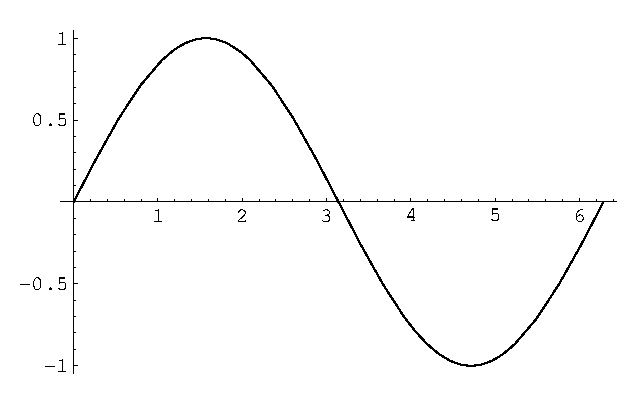
\includegraphics[width=1in]{plot1}}
\end{center}

\subsection*{Other Settings}

The file \textsf{localtexmf/tex/latex/pdfscreen/tuepdfscreen.cfg} contains all kind of settings, like margins and colours. You can create a copy of this file in your working directory and modify this copy.
\end{slidetop}

\begin{slidetop}
\setlength{\parskip}{0.2cm}
\section{Page Transitions}

You can choose other page transitions than the one you saw until now. The command to do this, is:

 \verb|\pagedissolve{<transition> <options>}|

The options depend on the transition. However, one option that you can always use is {\tt /D $n$}.
This sets the number of seconds that the transition lasts. The default page transition is creating using this command:

\begin{center}
\verb|\pagedissolve{R /D 0}|
\end{center}

The letter R stands for Replace, and /D 0 for a delay of 0 seconds. Before you use the command \verb|\pagedissolve|,
you should use a \verb|\newpage| command before starting the \hyperlink{slides}{\sf slide} or \hyperlink{slides}{\sf slidetop} environment.

Page transitions do not work really well in Linux/Unix (tested in Acrobat Reader 4 and 5).
\end{slidetop}

\begin{screen}
\newpage
\pagedissolve{Split /Dm /H /M /O}
\end{screen}

\begin{slide}
\subsection*{$\backslash$pagedissolve\{Split /Dm /H /M /O\}}

Two lines wipe over the screen and reveal the new page. These lines can move in a horizontal and vertical direction. Furthermore, they can move from the center towards the border (out), or the other way around (in).

\subsection*{Options}
\begin{descrsf}{/Dm {\it (dimension)}}
\item[/Dm {\it(dimension)}]
Determines whether the lines are horizontal or vertical. Possible values are /H (horizontal) and /V (vertical).

\item[/M {\it(motion)}]
Determines whether the lines move inward or outward. Possible values are
/I (in) or /O (out).
\end{descrsf}
\end{slide}

\begin{screen}
\newpage
\pagedissolve{Blinds /Dm /V}
\end{screen}

\begin{slide}
\subsection*{$\backslash$pagedissolve\{Blinds /Dm /V\}}

Multiple lines wipe over the screen and reveal the new page. These lines can be horizontal or vertical.

\subsection*{Options}
\begin{descrsf}{/Dm {\it (dimension)}}
\item[/Dm {\it(dimension)}]
Determines whether the lines are horizontal or vertical. Possible values are /H (horizontal) and /V (vertical).
\end{descrsf}
\end{slide}

\begin{screen}
\newpage
\pagedissolve{Box /M /O}
\end{screen}

\begin{slide}
\subsection*{$\backslash$pagedissolve\{Box /M /O\}}

A rectangle reveals the new page by moving from the center outward, or from the border inward.

\subsection*{Options}
\begin{descrsf}{/M {\it(motion)}}
\item[/M {\it(motion)}]
Determines whether the rectangle moves inward or outward. Possible values are
/I (in) or /O (out).
\end{descrsf}
\end{slide}

\begin{screen}
\newpage
\pagedissolve{Wipe /Di 270}
\end{screen}

\begin{slide}
\subsection*{$\backslash$pagedissolve\{Wipe /Di 270\}}

One line moves over the screen and reveals the next page. The direction of this line can be set using degrees. 0 degrees stands for "from left to right". Adding multiples of 90 degrees will change the direction counterclockwise.

\subsection*{Options}
\begin{descrsf}{/Di {\it (direction)}}
\item[/Di {\it (direction)}]
Specifies the direction of the line. Possible values are:\\
0 (from left to right)\newline
90 (from top to bottom) \newline
180 (from right to left) \newline
270 (from bottom to top)
\end{descrsf}
\end{slide}

\begin{screen}
\newpage
\pagedissolve{Dissolve}
\end{screen}

\begin{slide}
\subsection*{$\backslash$pagedissolve\{Dissolve\}}

Dissolves the old page, so the new page will become visible.

\subsection*{Options}

No options available.
\end{slide}

\begin{screen}
\newpage
\pagedissolve{Glitter /Di 0}
\end{screen}

\begin{slide}
\subsection*{$\backslash$pagedissolve\{Glitter /Di 0\}}

This is a combination of Dissolve and Wipe. The old page dissolves, but the effect moves in the specified direction.

\subsection*{Options}
\begin{descrsf}{/Di {\it (direction)}}
\item[/Di {\it (direction)}]
Specifies the direction of the dissolve effect. Possible values are:\\
0 (from left to right)\newline
90 (from top to bottom) \newline
180 (from right to left) \newline
270 (from bottom to top)
\end{descrsf}
\end{slide}

\begin{screen}
\newpage
\pagedissolve{R /D 0}
\end{screen}

\begin{slidetop}
\section{Images}

To include \hypertarget{images}{images} in your presentation, you should use the command
\verb|\includegraphics|. This command is defined in the package {\tt graphicx}.
The usage is:

\begin{verbatim}

\includegraphics[width=n]{imagefile}
\end{verbatim}

The width can be specified in units, like cm, mm or inch. But you can also specify any other \LaTeX\ length, e.g.
\verb|0.8\linewidth|. Imagefile is the file name of the image {\bf without extension}! Usually you start by generating an Encapsulated PostScript (EPS) file. You can convert this file to PDF using {\sf epstopdf} (TU/e MiK\TeX\ users can drag it on a shortcut called EPS2PDF on their desktop). By leaving out the file extension, PDF\LaTeX\ will choose the PDF version, and \LaTeX\ will choose the EPS version automatically.
\end{slidetop}

\begin{screen}

\newpage
\begin{slidetop}
\section*{Image example}

\[\int_0^{2\pi} \sin{x}\ {\textrm d}x\]

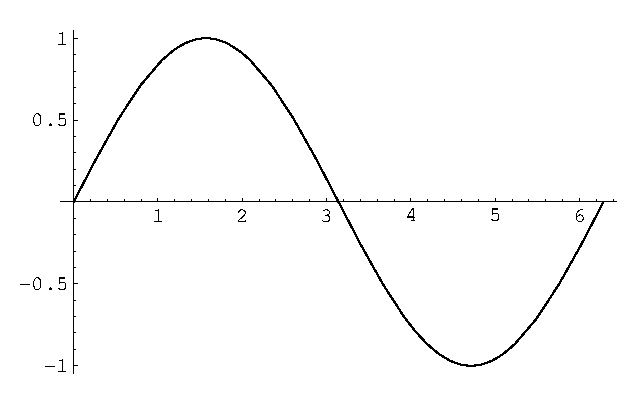
\includegraphics[width=0.8\linewidth]{plot1}
\end{slidetop}

\newpage
\addtocounter{page}{-1}
\pagedissolve{Wipe /Di 0}

\begin{slidetop}
\section*{Image example}

\[\int_0^{2\pi} \sin{x}\ {\textrm d}x = 2\]

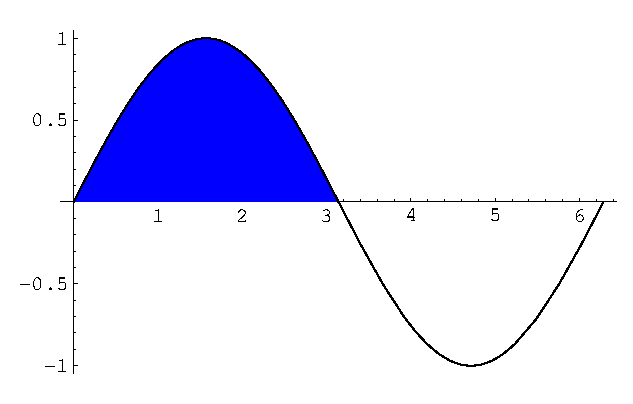
\includegraphics[width=0.8\linewidth]{plot2}
\end{slidetop}

\newpage
\addtocounter{page}{-1}
\begin{slidetop}
\section*{Image example}

\[\int_0^{2\pi} \sin{x}\ {\textrm d}x = 2 - 2\]

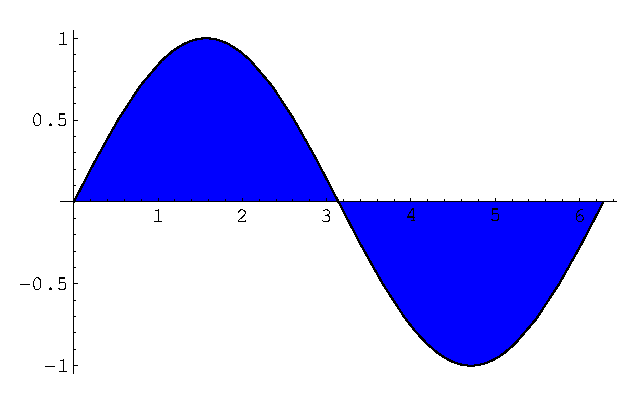
\includegraphics[width=0.8\linewidth]{plot3}
\end{slidetop}

\newpage
\pagedissolve{R /D 0}
\addtocounter{page}{-1}
\end{screen}

\begin{slidetop}
\section*{Image example}

\[\int_0^{2\pi} \sin{x}\ {\textrm d}x = 2 - 2 = 0\]

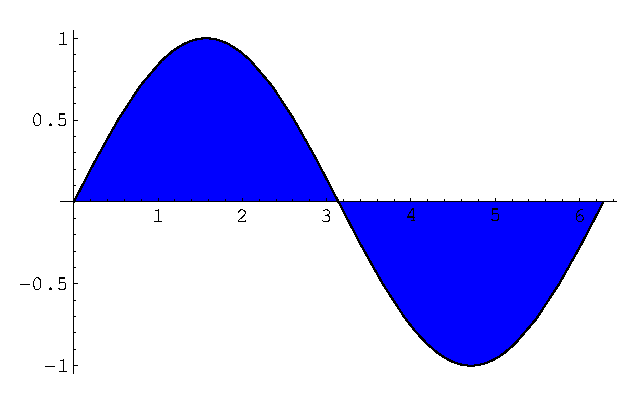
\includegraphics[width=0.8\linewidth]{plot3}
\end{slidetop}


\begin{slidetop}
\section{Captions and References}
\setlength{\parindent}{0cm}
\setlength{\parskip}{0.2cm}

Because the {\sf slide} and {\sf slidetop} environments are implemented as minipages, the {\sf figure} and {\sf table} environments cannot be used. Most of the people do not regard this as a problem, but they regret the fact that the \verb|caption| command can no longer be used. This means that you cannot refer to an image or a table. We solved this problem in TU/ePDFScreen by defining two new commands: \verb|\tablecaption| and \verb|\figcaption|.
These commands should be used instead of the  \verb|\caption| command:\newline

\begin{verbatim}
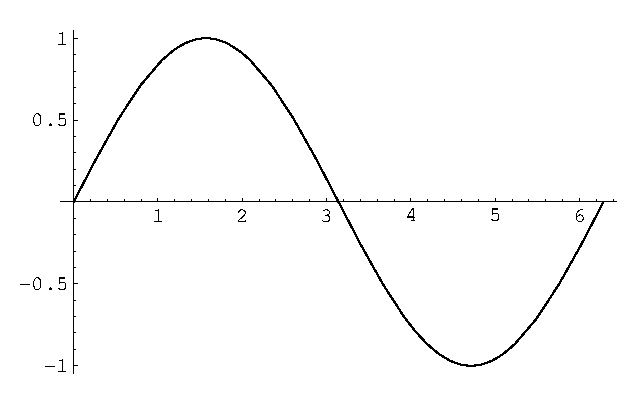
\includegraphics[width=0.5\linewidth]{plot1}
\figcaption{a sine function}
\label{fig:sine}
\end{verbatim}

You can still use the command \verb|\ref| to create a reference to this image.
\end{slidetop}

\begin{slidetop}
\setlength{\parindent}{0cm}
\setlength{\parskip}{0.2cm}

On this page you will see an example of the usage of \verb|\figcaption| and \verb|\tablecaption|. Look at the source code for more details.

\begin{tabularx}{\linewidth}{XX}

\centering
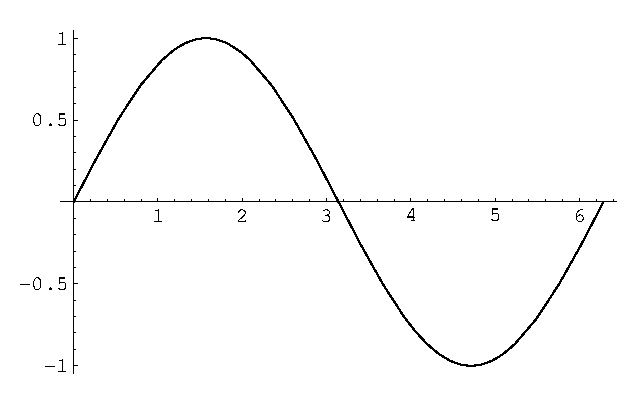
\includegraphics[width=0.6\linewidth]{plot1}
\figcaption{Een sine function}
\label{fig:sine}

&

\centering
\begin{tabular}{|c|c|}
\hline
\multicolumn{2}{|c|}{A Table}\\
\hline
Mick & Keith \\
Charlie & Ron \\
\hline
\end{tabular}
\tablecaption{Some random names.}
\label{table:tableexample}

\end{tabularx}

For the figure we used the  \verb|\figcaption| command, for the table we used the \verb|\tablecaption| command. Creating a reference to figure \ref{fig:sine} or table \ref{table:tableexample} can be done using \verb|\ref|.\newline

In the source code you might see the usage of a {\sf tabularx} environment. We used this only to be able to put the figure and the table next to each other. It has nothing to do with the caption commands.

\end{slidetop}

\begin{slidetop}
\setlength{\parskip}{0.2cm}
\hypertarget{printhandouts}{\section{Printing Handouts}}

Since TU/ePDFScreen is written specifically for PDF\LaTeX, you have to use Adobe Acrobat (Reader) for both viewing and printing your slides. For printing you can use the keyboard shortcut CTRL+P. If you want to print the slides on A4 paper, you do not have to change any print settings. Make sure that you have at least Adobe Acrobat version 5, because in version 4 some fonts are printed incorrectly.

If have pages in your presentation that you don't want to print, you should put them in a {\sf screen} environment:

\verb|\begin{screen}| $\ldots$ {\it some slides} $\ldots$ \verb|\end{screen}|

This means that the page numbers on the printed slides will be different from the page numbers of the presentation. To solve this problem, read the section on \hyperlink{pagenumbering}{pagenumbering}.
\end{slidetop}

\begin{slidetop}
\subsection*{Multiple slides on one page}

\begin{wrapfigure}{r}{0.4\linewidth}
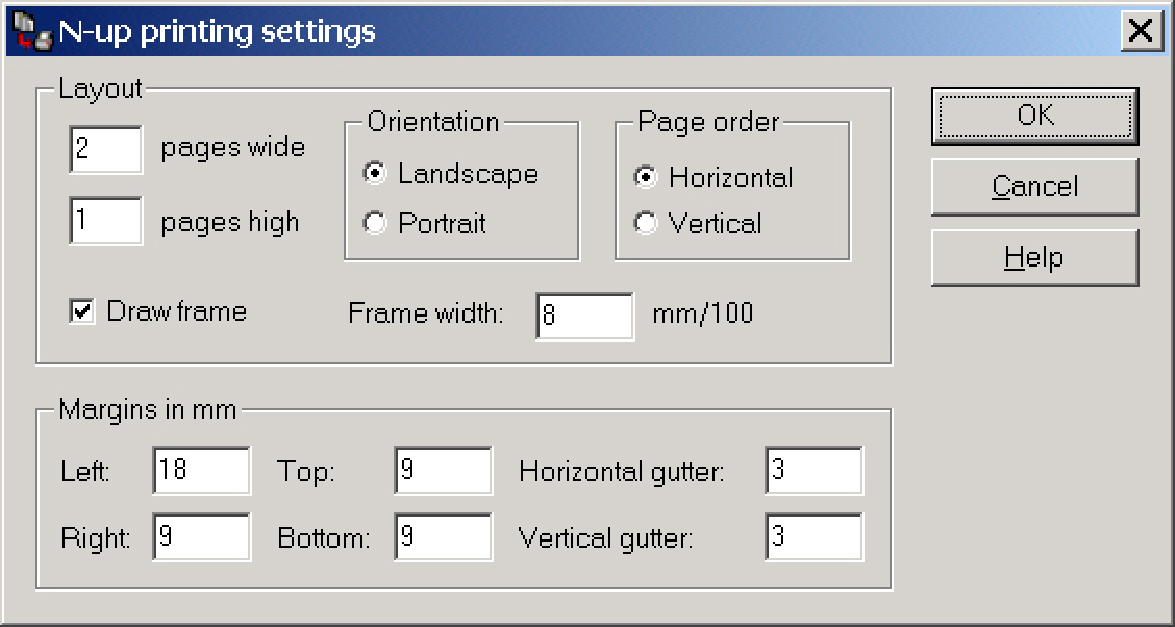
\includegraphics[width=\linewidth]{psnup}
\figcaption{N-up in PrintFile}
\label{psnup}
\end{wrapfigure}
Modern printer drivers (HP printers in Windows 2000 or XP) support printing multiple sheets on one page. Just click the Properties button in the Print dialog. If your printer driver does not support multiple sheets on one page, you can always generate pure PostScript.
To generate PostScript from any application you can install the QMS Colorscript 1000 printer. The drivers are available on any Windows CD-ROM. Do not specify any port, but choose "Print to file (FILE:)". This will make a dialog pop up every time you print a file to this printer. Save this file on your local disk. Then use PrintFile, which comes with your TU/e MiK\TeX\ distribution, to print this file. First select the file, then press {\bf\sf Settings $\longrightarrow$ PostScript $\longrightarrow$ Enable n-up printing}. Then, also in the Settings dialog, press the N-up button. This will bring up the dialog shown in figure \ref{psnup}.


\end{slidetop}

\begin{screen}
\newpage
\pagedissolve{Wipe /Di 0}
\end{screen}

\begin{slidetop}
\section{Revealing slides in multiple steps}
\begin{itemize}
\item PowerPoint users might miss the animation feature that makes objects move into the slide.
      This is not possible in TU/ePDFScreen.

\pause

\item However, as you can see, you can simulate this kind behaviour. There are two ways to do this.

\pause

\item The first way is just to create the complete page (use {\sf slidetop} environment). When the page is finished, make as many copies of this page as necessary, and remove one more statement each time. Put all pages except the last, complete page in a {\sf screen} environment to prevent them from being printed in \hyperlink{handouts}{handouts} mode.
Please note that page numbering and chapter numbering should manually be controlled to prevent these number from being increased. See \hyperlink{pagenumbering}{pagenumbering} for more information.
\end{itemize}
\end{slidetop}

\begin{screen}
\newpage
\end{screen}

\begin{slidetop}
\begin{itemize}
\item the second way, which is used here, is easier to use. Just put a \verb|\pause| command whenever you want a break. After running PDF\LaTeX\ you still will not notice anything in the resulting PDF file. You have to run a postprocessor called {\sf AddPause}. This program will bring up an Open File dialog so you can select your PDF file. AddPause will add the breaks and generate another PDF file without the break effects (you can use this for handouts).

Please note that AddPause uses PPower4, a Java program written by Klaus Guntermann. Therefore you need Java to run it. This means that you have to install it manually on systems without Java (like Windows XP).
\end{itemize}
\end{slidetop}

\begin{screen}
\newpage
\pagedissolve{R /D 0}
\end{screen}

\begin{slidetop}
You can always contact:

\begin{center}
\tuebox{
\begin{tabular}{cc}
Marko Boon & Wil Kortsmit \\
\href{mailto:marko@win.tue.nl}{marko@win.tue.nl} & \href{mailto:rcwil@win.tue.nl}{rcwil@win.tue.nl} \\
HG 9.09 & HG 9.83 \\
2989 & 4587
\end{tabular}
}
\end{center}
\begin{itemize}
\item for questions concerning TU/ePDFScreen
\item for questions regarding MiK\TeX\ or \LaTeX
\item to get a free copy of the latest TU/e MiK\TeX\ CD-ROM
\end{itemize}

\vspace{-1em}
\begin{center}

\includegraphics[width=0.3\textwidth]{miktexcd}
\end{center}

\end{slidetop}

\end{document}
